\section{Evidence supporting the design}\label{sec:evidence}
This appendix presents the corpus checks and objective-evaluation measurements supporting the design, together with their limits. We evaluate fixed candidate routes and finite matrix constructions, without new solver searches or optimality proofs.

\subsection{Corpus and matrix checks}
% Internal experiment record: /home/onyr/code/phd/numerical-checker-contracts-investigation/results/s120-sintef/protocol.json, protocol-addendum.json, sources.json, summary.json, supplementary-results.json and reproducibility.json. Frozen experiment revision: 982044f967f3a689dcd10847894bef326b8d14b8. Source corpus revision: eca336ff4b087f5c2f7b9ac7c2ab33668ff7af2b.
We capture the official SINTEF instance and detailed-solution sources in October 2026 and compare 364 linked official route files, covering 356 distinct instances, with 468 MAMUT incumbent files from the recorded corpus snapshot. The official detailed-route coverage concerns instances with 100 to 1000 customers. The MAMUT corpus also includes the 25- and 50-customer variants. These are separate coverage denominators, rather than a claim that an official detailed route was obtained for every local instance.

We evaluate each candidate with 7 numerical recipes: submitted-order flat binary64, canonical flat binary64, canonical grouped binary64, exact arithmetic over binary64 values, 128-significant-digit decimal arithmetic over the same binary64 values, and 128-significant-digit coordinate-distance arithmetic in submitted and canonical route order. The last 2 recipes change the distance source as well as the arithmetic. They are geometric diagnostics, rather than exact evaluation of the published binary64 matrix. The comparisons use no feasibility epsilon. We preserve each recipe's objective and temporal recurrence separately instead of inferring feasibility from its final objective.

All 364 official route files and all 468 MAMUT incumbents pass all 7 tested recipes. We also compare every directed entry of the 468 stored matrices with the square-root construction, \id{hypot}, and 128-significant-digit decimal square roots rounded once to binary64. All 133,115,068 entries agree on the recorded x86-64 host with Python 3.13.13 and glibc 2.42. Separate fresh processes reproduce the matrix and route-result outputs byte for byte. This is recorded-environment evidence, rather than cross-platform certification.

Rounding the exact-binary objective once changes 397 of the 468 serialized MAMUT costs. Hence agreement on the feasibility of the retained candidates does not imply agreement on result serialization. These observations also do not prove that every possible route has identical feasibility under the recipes or identify SINTEF's private arithmetic uniquely.

% Internal source associations: /home/onyr/code/phd/numerical-checker-contracts-investigation/results/s120-sintef/source-context.json, identity-audit.json and supplementary-results.json.
We distinguish source-association issues from arithmetic differences. Ten table claims have explicit source warnings with higher linked alternatives, and \id{R1_10_7} retains an unresolved table/link discrepancy. Two official route candidates, \id{R1_10_3} and \id{R1_10_6}, improve on the MAMUT incumbents under the compared canonical and exact recipes. Compact or incomplete downloaded route headers require normalization in derived records while preserving raw source bytes. These curation tasks remain outside the specification draft.

\subsection{Objective-evaluation runtime}
% Internal experiment: /home/onyr/code/phd/numerical-checker-contracts-investigation/scripts/s124_cost_runtime.py, s124_cost_runtime_validate.py and s124_cost_runtime_report.py. Raw evidence: newresults/s124-cost-runtime/{inputs,protocol,run1,run2,validation,comparison,report-artifacts}.json. Unchanged timing kernels: scripts/s120_cost_runtime.py. Source corpus revision: eca336ff4b087f5c2f7b9ac7c2ab33668ff7af2b. Session s124, 26 October 2026.
We measure all 296 SINTEF incumbents at the 5 requested customer counts: 56 instances with 100 customers and 60 instances each with 400, 600, 800 and 1000 customers. This replaces the earlier 12-instance, 1000-customer timing panel with a complete census at these sizes. The 25-, 50- and 200-customer instances are outside this runtime experiment. We verify every descriptor and incumbent against the same immutable corpus revision used for the corpus checks. All included route lists are already canonical.

We retain the 9 Python objective implementations from the earlier experiment and measure them in 2 sequential fresh processes. Each instance, implementation and scope has 5 warm-up calls and 9 measured blocks, with a 20 ms calibration target. We shuffle instance order and block order with seed 20261026. The measurements use an Intel i7-12700H with Python 3.13.13. Garbage collection is disabled during measured blocks and restored afterwards. CPU affinity spans CPUs 0 to 19 without pinning, so scheduling and background load remain sources of variation. We load and prepare 1 matrix at a time to bound memory use.

The loaded-input scope starts with binary64 matrices and canonical routes in memory. It includes route traversal and any per-call numerical conversion. The prepared-operand scope starts with gathered and preconverted arc operands. Loading, hashing, structural validation, temporal checking, geometric construction, canonical sorting and output serialization are outside both timers. The coordinate Decimal diagnostic is an explicit exception to loaded-matrix traversal: it uses prepared coordinate-distance buffers in both scopes and changes the distance source. Submitted flat and canonical flat use the same operation order in this corpus. Grouped Python \id{sum} is an interpreter-dependent diagnostic distinct from the explicit grouped left fold.

\begin{figure}[htbp]
\centering
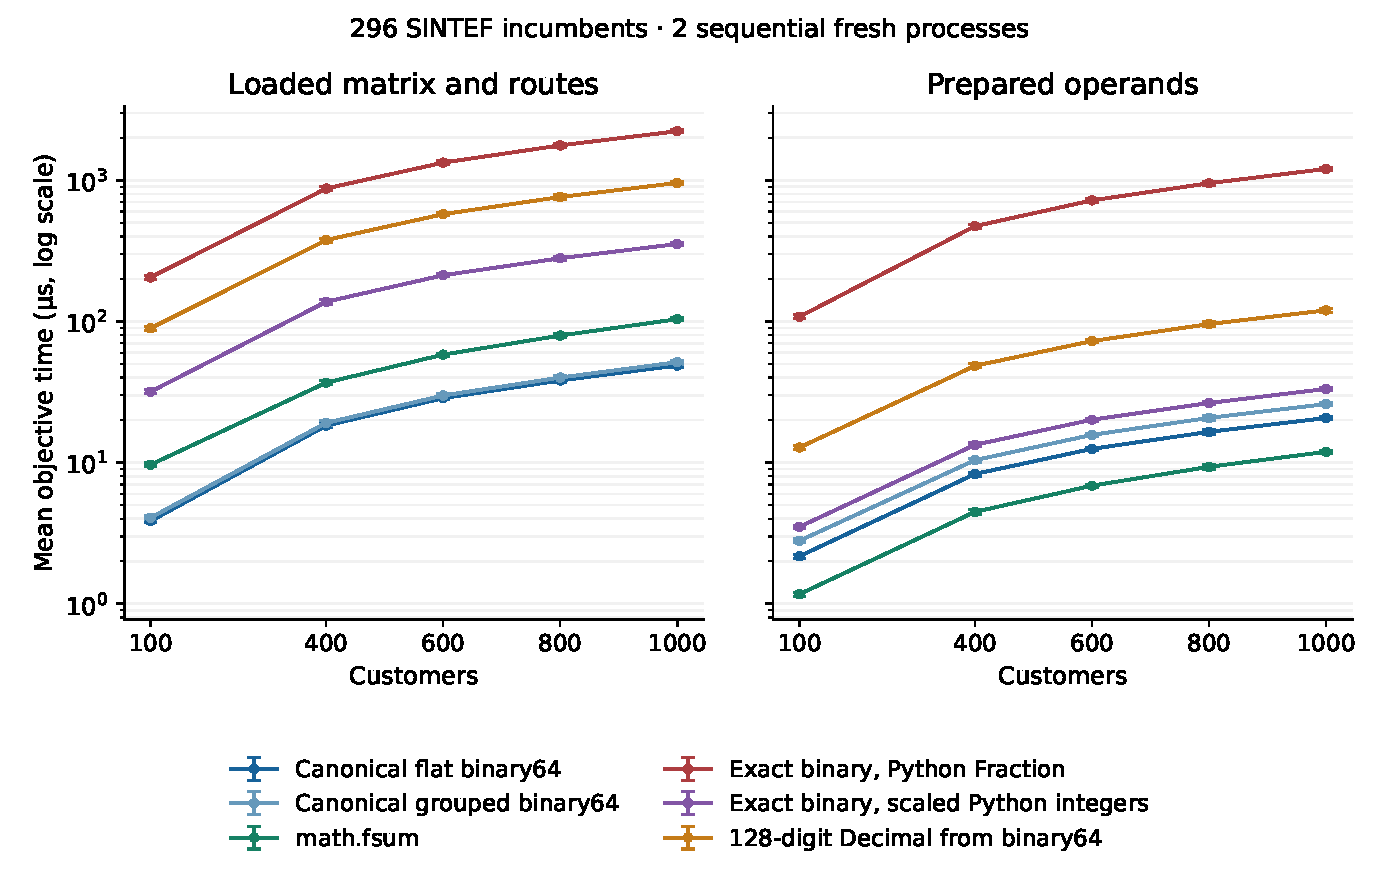
\includegraphics[width=\linewidth]{figures/objective-runtime-by-size.pdf}
\caption{Objective-evaluation time against customer count for 6 principal implementations, covering every instance at each requested size. Points give equal weight to every instance and each process within a size. The vertical axis is logarithmic. Error bars span the 2 process means, rather than a confidence interval. The full results for all 9 implementations are in Tables~\ref{tab:runtime-loaded} and~\ref{tab:runtime-prepared}.}\label{fig:objective-runtime}
\end{figure}

\begin{table}[htbp]
\centering\small
\begin{tabularx}{\linewidth}{@{}Xrrrrr@{}}
\toprule
Objective implementation & 100 & 400 & 600 & 800 & 1000\\
\midrule
Submitted flat binary64 & 3.9 & 18.4 & 28.7 & 38.4 & 49.1\\
Canonical flat binary64 & 3.9 & 18.3 & 28.6 & 38.2 & 48.7\\
Grouped binary64, explicit loops & 4.1 & 19.1 & 29.9 & 40.0 & 51.4\\
Grouped Python \id{sum} & 10.9 & 42.3 & 66.2 & 87.0 & 110.1\\
\id{math.fsum} & 9.7 & 36.8 & 58.2 & 79.4 & 103.7\\
Exact binary, Python \id{Fraction} & 205.1 & 873.0 & 1332.2 & 1763.4 & 2223.1\\
Exact binary, scaled integers & 31.8 & 137.6 & 212.2 & 280.0 & 353.5\\
128-digit Decimal from binary64 & 89.3 & 376.7 & 574.7 & 760.3 & 956.5\\
128-digit coordinate Decimal cache$\dagger$ & 19.8 & 77.4 & 116.8 & 153.6 & 191.1\\
\bottomrule
\end{tabularx}
\caption{Loaded matrix and routes: mean objective-evaluation time in $\mu$s per complete solution, by customer count. Each size gives equal weight to every instance and each process. $\dagger$The coordinate Decimal diagnostic uses prepared distances in both scopes and changes the distance source.}\label{tab:runtime-loaded}
\end{table}

\begin{table}[htbp]
\centering\small
\begin{tabularx}{\linewidth}{@{}Xrrrrr@{}}
\toprule
Objective implementation & 100 & 400 & 600 & 800 & 1000\\
\midrule
Submitted flat binary64 & 2.2 & 8.3 & 12.5 & 16.5 & 20.7\\
Canonical flat binary64 & 2.2 & 8.3 & 12.5 & 16.5 & 20.7\\
Grouped binary64, explicit loops & 2.8 & 10.4 & 15.7 & 20.7 & 26.0\\
Grouped Python \id{sum} & 1.7 & 5.4 & 8.0 & 10.4 & 12.9\\
\id{math.fsum} & 1.2 & 4.5 & 6.9 & 9.3 & 11.9\\
Exact binary, Python \id{Fraction} & 107.9 & 472.4 & 719.7 & 951.7 & 1202.5\\
Exact binary, scaled integers & 3.5 & 13.4 & 20.1 & 26.4 & 33.3\\
128-digit Decimal from binary64 & 12.8 & 48.5 & 72.6 & 95.7 & 119.8\\
128-digit coordinate Decimal cache$\dagger$ & 19.8 & 77.4 & 117.1 & 153.7 & 190.7\\
\bottomrule
\end{tabularx}
\caption{Prepared operands: mean objective-evaluation time in $\mu$s per complete solution, by customer count. Each size gives equal weight to every instance and each process. $\dagger$The coordinate Decimal diagnostic uses prepared distances in both scopes and changes the distance source.}\label{tab:runtime-prepared}
\end{table}

\begin{table}[htbp]
\centering\small
\begin{tabular}{@{}rrrrrr@{}}
\toprule
Customers & Instances & Preparation (ms) & Matrix scan (ms) & Exponent $q$ & Total bits\\
\midrule
100 & 56 & 3.6 & 2.2 & 51, 52 & 61--63\\
400 & 60 & 43.7 & 36.6 & 52 & 64--66\\
600 & 60 & 95.1 & 83.9 & 52 & 65--67\\
800 & 60 & 160.1 & 148.7 & 52 & 66--68\\
1000 & 60 & 248.5 & 234.2 & 52 & 66--68\\
\bottomrule
\end{tabular}
\caption{Preparation outside the objective timers. The full-matrix scale scan is included in preparation. Bit counts concern the observed incumbent totals at each matrix's common binary scale, rather than all possible solver intermediates.}\label{tab:runtime-preparation}
\end{table}


At 1000 customers, exact scaled-integer evaluation averages 353.5~$\mu$s from loaded inputs and 33.3~$\mu$s from prepared operands, compared with 2223.1 and 1202.5~$\mu$s for \id{Fraction}. Canonical flat binary64 takes 48.7 and 20.7~$\mu$s in the same scopes. Hence the representation and conversion boundary materially affect the measured cost of satisfying the exact objective contract.

Preparation includes the full-matrix binary-scale scan and the construction of gathered and converted route buffers. Table~\ref{tab:runtime-preparation} reports its cost separately, outside both evaluation timers. It can be amortized across repeated evaluations. We do not measure a solver that preconverts and stores every matrix entry as an integer. The observed bit counts concern retained incumbent totals, without establishing a range bound for every possible route, pricing label or proof intermediate.

The full matrices require scale exponents 51 or 52, and the observed scaled incumbent totals occupy 61 to 68 bits. Some observed totals already exceed a signed 64-bit accumulator at the matrix's common scale, so a native implementation requires explicit range checks or wider arithmetic.

Before and after timing, each implementation returns the same objective in both scopes. Independent replay compares all numerical outputs with the frozen route-audit results or, for the interpreter-dependent grouped diagnostic, an independent built-in-sum expression. The exact scaled-integer and rational implementations agree on every incumbent objective, and all implementation outputs agree across the 2 processes. Raw measured blocks, iteration counts, per-instance timings, source identities and input hashes are retained with the experiment.

The generator-based \id{fsum} wrapper and the tight flat traversal charge different Python data-access costs in the loaded-input scope. We therefore interpret the measurements as costs of these implementations and their preparation choices, rather than an intrinsic speed ordering of numerical contracts. The experiment measures no Linear Programming (LP), pricing, dominance or complete proof performance. Process-to-process timing variation is descriptive and does not establish cross-platform performance.

These observations support making exactness an outcome contract with alternative efficient implementations. They do not justify requiring generic rational arithmetic inside every solver. The exact-integer results also show why a \id{Fraction} microbenchmark is not a universal cost estimate for exact binary evaluation. An integration pilot is still required before estimating certification overhead for an existing BPC engine.

\FloatBarrier
\subsection{Native implementation, complete checking and Python integration}\label{sec:native-evidence}
% Internal experiment: /home/onyr/code/phd/numerical-checker-contracts-investigation/native/s124/{dyadic.hpp,bindings.cpp,CMakeLists.txt,build.py,reference.py} and scripts/s124_native_{runtime,conformance,validate,report}.py. Results: newresults/s124-native/. The original Python census in newresults/s124-cost-runtime/ is preserved unchanged.
We extend the objective experiment with a native implementation and complete retained-solution checking on the same 296 instances. We retain all earlier Python objective measurements, tables and figures. This pilot uses C++20 with GCC/G++ 15.2.0, Boost 1.89.0 and pybind11 3.1.0 on the same x86-64 host with Python 3.13.13. We follow the existing Kayros/PyVRP pattern of an owned native data model behind pybind11 bindings, without changing either solver or the production MAMUT library.

\subsubsection{Exact arithmetic, range bounds and boundary behavior}
We decode each finite nonnegative binary64 quantity into an integer significand and a binary exponent, including subnormals and signed zero. We select a common scale $2^q$ over every arc cost, time-window bound and service duration. This produces exact integer operands without floating-point multiplication or rounding. Let $A$, $E$, $L$ and $S$ denote the maximum scaled arc cost, earliest time, latest time and service duration. For an instance with $n$ customers, we use the conservative bound
\[
    B = \max\!\left\{2nA,\ E+(n+1)(A+S)\right\}.
\]
Every structurally valid solution has at most $n$ nonempty routes and hence at most $2n$ arcs in total. A route has at most $n+1$ arcs and $n$ customer service contributions. The historical pilot allowed an additional service term in its conservative bound. Under this specification that depot term is zero. Expanding the waiting recurrence bounds every arrival or departure by the largest earliest time plus the accumulated arc and service contributions. Hence $B$ bounds the objective and temporal intermediates for this instance, rather than only the retained incumbent. We also require $L$ to fit the chosen representation.

When $\max\{B,L\}\leq 2^{127}-1$, the prototype uses Boost's fixed-width unsigned 128-bit storage with a reserved sign bit and explicit checked additions. Otherwise, it prepares arbitrary-precision integer operands. A checked-add overflow also triggers an arbitrary-precision retry before a result is accepted. Capacity checks compare each demand with remaining capacity before addition. The pilot supports resource integers that are exactly representable in binary64 and lie between 0 and the signed 64-bit maximum, and caps the customer count at $10^6$ subject to available memory. It rejects unsupported resource widths explicitly. This supported domain is a restriction of the general reference, rather than a claim to implement every static input accepted by the specification.

The boundary suite checks every finite binary64 exponent class, subnormal bit positions, mixed-exponent sums, signed zero, nonfinite rejection, exact objectives beyond finite binary64, and checked-overflow fallback. It compares feasibility and exact costs with the frozen Python reference on depot/service, time-window, capacity, fleet and structural witnesses. In particular, the rounded checker accepts a constructed deadline case that the exact checker rejects. We also check native ownership of matrix and route data, so later mutations of the supplied Python objects cannot silently change the prepared model. The independent suite contains 2496 passing checks, and 67 standalone core checks pass under address and undefined-behavior sanitizers with standard-library assertions. These tests are evidence for the recorded build, rather than certification of every compiler or platform.

\subsubsection{Measurement scopes and integration boundaries}
We run 2 sequential fresh processes over all 296 instances, with 5 warm-ups and 9 randomized measured blocks per cell, a 20 ms calibration target and seed 2026102607. The native extension uses optimized C++20 without fast-math or floating-point contraction, and without a host-specific architecture flag. We measure 6 native operations: flat binary64 objective evaluation, exact objective evaluation with per-arc conversion or a prepared integer matrix, and complete solution checking with each of those 3 arithmetic paths. The rounded full checker is a separately identified numerical diagnostic.

The complete checker validates nonempty routes, exact customer coverage, duplicates, fleet size, capacity, depot initialization, service durations, all customer and return time windows, and the objective. Input parsing, instance validation, matrix packing and numeric preparation remain outside the solution-checking timers. Table~\ref{tab:native-preparation} reports those preparation costs separately. The native model owns both a binary64 matrix and its exact integer materialization. The full Python reference additionally parses the original JSON tokens and constructs a Fraction matrix, so its preparation column includes different work.

For each native operation, we measure a C++ batch and repeated Python calls through pybind11. The C++ timer runs inside the batch, excluding its single Python binding call and result wrapping. A compiler signal fence and an independently checked result checksum prevent the benchmark from discarding the repeated evaluations. Scalar binding calls include per-call dispatch and native-result wrapping. They retain the Global Interpreter Lock (GIL), while a batch releases it once around the repeated native work. Separate measurements add conversion of Python route lists on every complete check, then extraction and normalization of the exact Python hierarchical ranking key. The frozen Python reference also performs its existing canonical sorting and returned-route copies. These are measured implementation boundaries, rather than identical serialization pipelines.

\begin{figure}[htbp]
\centering
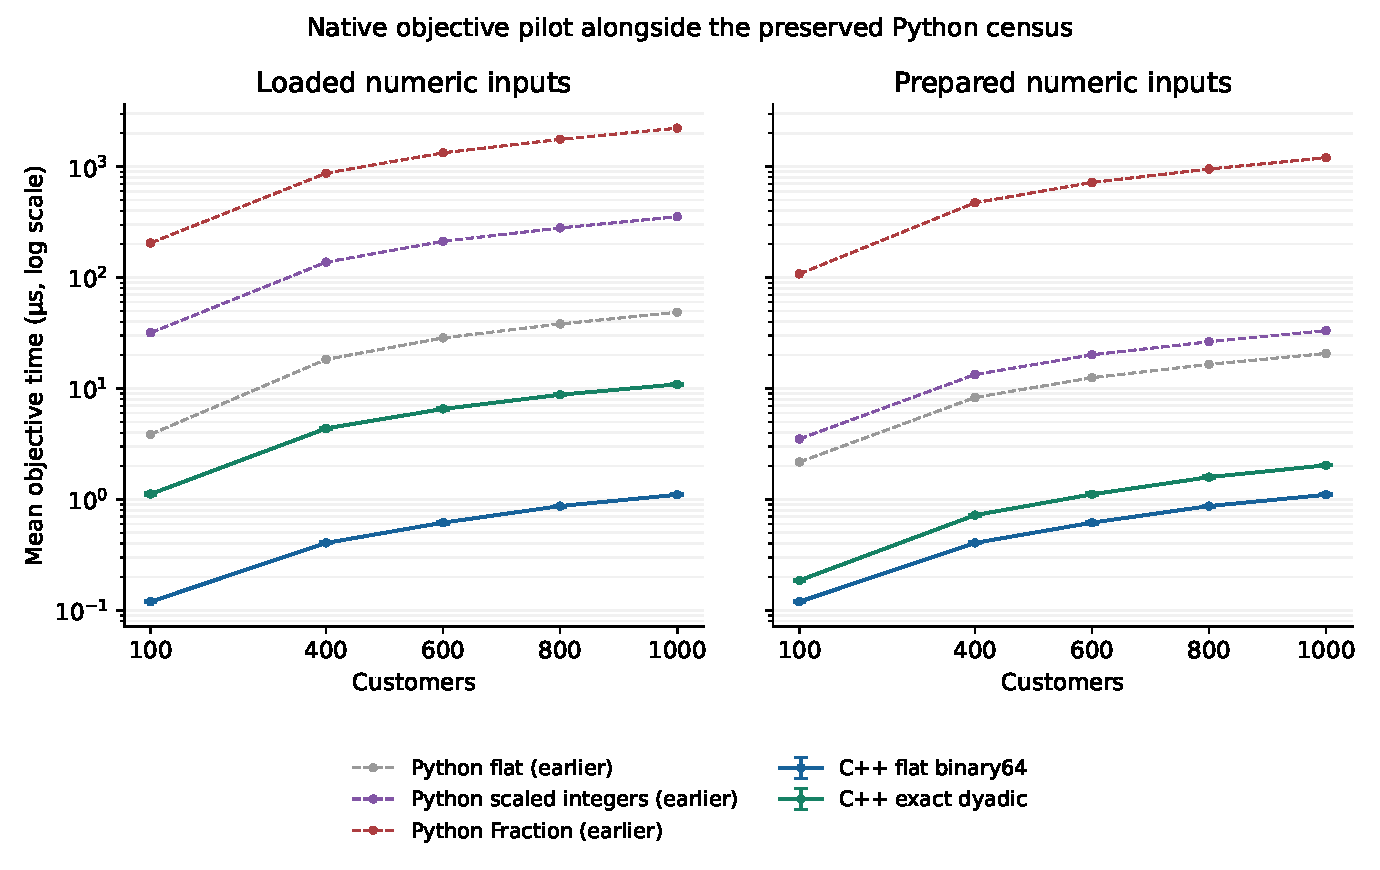
\includegraphics[width=\linewidth]{figures/native-objective-by-size.pdf}
\caption{Native objective evaluation alongside the preserved Python census, with logarithmic time axes. Native error bars span the 2 process means. The native prepared scope traverses a full integer matrix, while the earlier Python prepared scope reduces gathered route operands. Dashed Python curves retain the earlier processes and provide implementation context rather than simultaneous paired comparisons.}\label{fig:native-objectives}
\end{figure}

\begin{figure}[htbp]
\centering
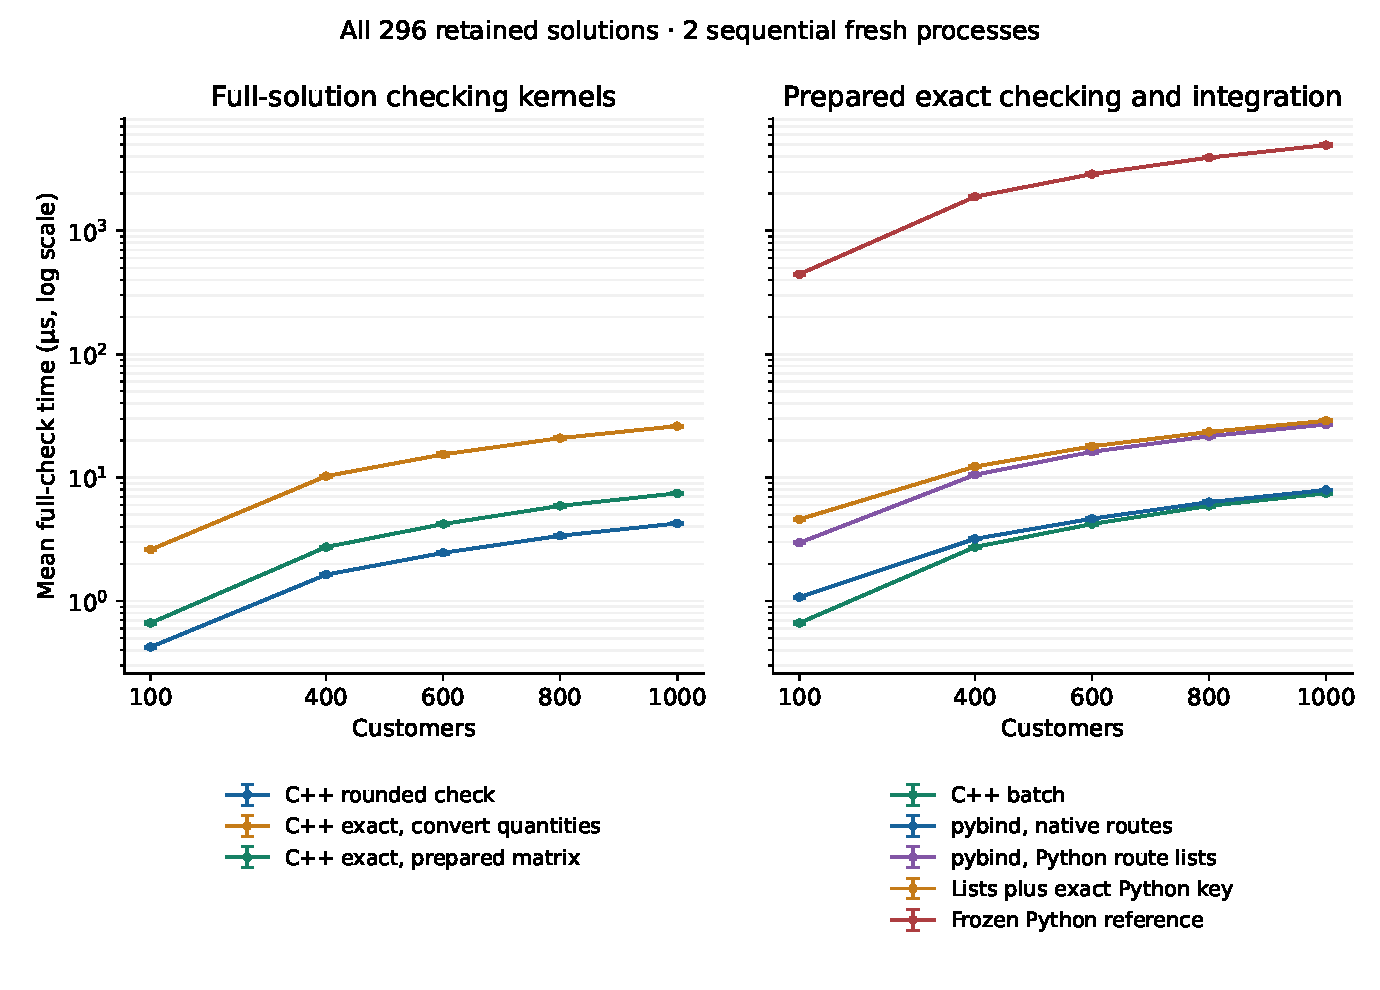
\includegraphics[width=\linewidth]{figures/native-checking-by-size.pdf}
\caption{Complete checking and Python integration on every retained solution at each requested size. The left panel compares concrete native arithmetic paths. The right panel separates native batches, scalar bindings, route-list conversion, exact-key extraction and the frozen Python reference. Error bars span process means and are not confidence intervals.}\label{fig:native-checking}
\end{figure}

\begin{table}[htbp]
\centering\small
\begin{tabularx}{\linewidth}{@{}Xrrrrr@{}}
\toprule
Implementation & 100 & 400 & 600 & 800 & 1000\\
\midrule
Flat binary64 objective & 0.120 & 0.405 & 0.618 & 0.871 & 1.102\\
Exact objective, convert arcs & 1.117 & 4.363 & 6.540 & 8.786 & 10.896\\
Exact objective, prepared matrix & 0.186 & 0.722 & 1.111 & 1.588 & 2.031\\
Rounded full check & 0.424 & 1.636 & 2.459 & 3.380 & 4.253\\
Exact full check, convert quantities & 2.606 & 10.277 & 15.412 & 20.899 & 26.139\\
Exact full check, prepared matrix & 0.664 & 2.739 & 4.209 & 5.902 & 7.467\\
\bottomrule
\end{tabularx}
\caption{Pure C++ batches: mean time in $\mu$s per complete solution, by customer count. The timer excludes the single batch binding call and result wrapping. Rounded checks are diagnostics with different numerical semantics.}\label{tab:native-kernels}
\end{table}

\begin{table}[htbp]
\centering\small
\begin{tabularx}{\linewidth}{@{}Xrrrrr@{}}
\toprule
Implementation & 100 & 400 & 600 & 800 & 1000\\
\midrule
Flat binary64 objective & 0.517 & 0.851 & 1.095 & 1.353 & 1.593\\
Exact objective, convert arcs & 1.530 & 4.797 & 7.005 & 9.208 & 11.348\\
Exact objective, prepared matrix & 0.584 & 1.135 & 1.534 & 2.024 & 2.462\\
Rounded full check & 0.827 & 2.054 & 2.918 & 3.856 & 4.722\\
Exact full check, convert quantities & 3.021 & 10.780 & 15.948 & 21.398 & 26.661\\
Exact full check, prepared matrix & 1.076 & 3.189 & 4.647 & 6.329 & 7.938\\
Prepared exact check, Python route lists & 2.966 & 10.539 & 16.202 & 21.649 & 26.951\\
Route lists and exact Python ranking key & 4.597 & 12.288 & 17.928 & 23.438 & 28.891\\
Frozen Python reference full check & 444.597 & 1884.382 & 2875.155 & 3912.013 & 4939.869\\
\bottomrule
\end{tabularx}
\caption{Python integration: mean time in $\mu$s per complete solution. The first 6 rows call the same native kernels through pybind11 on prepared native route objects. The final rows add route-list conversion, exact-key extraction, or use the frozen Fraction reference, whose sorting and output copies are included.}\label{tab:native-integration}
\end{table}

\begin{table}[htbp]
\centering\small
\begin{tabular}{@{}rrrrrr@{}}
\toprule
Customers & NumPy (ms) & Native (ms) & Reference (ms) & Payload (MiB) & Bound bits\\
\midrule
100 & 0.20 & 0.10 & 22.5 & 0.23 & 66--67\\
400 & 3.20 & 0.96 & 400.3 & 3.68 & 70\\
600 & 6.89 & 2.00 & 913.0 & 8.27 & 71\\
800 & 11.63 & 3.46 & 1720.2 & 14.69 & 72\\
1000 & 18.06 & 5.34 & 2813.5 & 22.93 & 73\\
\bottomrule
\end{tabular}
\caption{Preparation outside solution-checking timers. NumPy packs the already loaded Python matrix. Native preparation owns, validates and converts that matrix and the temporal/resource arrays. Reference preparation additionally parses JSON tokens and constructs the full Fraction matrix. Payload counts the native binary64 and fixed-width matrix buffers, excluding Python objects and allocation overhead. Bound bits cover the conservative objective/temporal bound, rather than only the retained incumbent.}\label{tab:native-preparation}
\end{table}


All 296 instances admit the checked fixed-width path, with conservative objective/temporal bounds occupying 66 to 73 bits. At 1000 customers, the prepared native exact objective averages 2.031~$\mu$s, compared with 1.102~$\mu$s for flat binary64. The corresponding complete checks average 7.467 and 4.253~$\mu$s. Converting quantities during each exact complete check raises its mean to 26.139~$\mu$s. These within-C++ measurements quantify the costs of the arithmetic and preparation choices on the recorded inputs.

At the same size, the prepared exact complete check takes 7.938~$\mu$s through pybind11 with a retained native route object, 26.951~$\mu$s when Python route lists are converted on every call, and 28.891~$\mu$s including extraction of the exact Python ranking key. The frozen Fraction reference takes 4939.869~$\mu$s, including its existing canonical sorting and returned-route copies. Hence the route and result boundary contributes measurable work even when the native checking kernel is small. The native matrix buffers occupy 22.93~MiB at this size, so the timing benefit of full integer preparation also has a storage cost.

\subsubsection{Coverage and remaining portability obligations}
Every native exact objective and complete-check result agrees with the independent frozen route audit and the Python reference on the retained candidates. We independently replay input identities, common scales, instance-wide range bounds, batch checksums and raw timing aggregates. The published artifacts preserve source, build, dependency and input identities. The original Python objective data and exports remain unchanged.

This experiment measures a complete checker and an actual Python/native handoff in the investigation repository. It does not measure production-library loading, sidecar resolution, metadata hashing, JSON serialization, solver search, pricing or proof certification. The results therefore address the native arithmetic and integration pilot requested in point 7 without establishing complete downstream integration or cross-platform equivalence. Actual builds and conformance runs on other operating systems, architectures and Python interfaces remain necessary before making those portability claims.

